%%%%%%%%%%%%%%%%%%%%%%%%%%%%%% -*- Mode: Latex -*- %%%%%%%%%%%%%%%%%%%%%%%%%%%%
%% 00-00.tex -- IEEE Software paper
%% Author          : Hongbing Kou
%% Created On      : Mon Sep 23 11:52:28 2002
%% Last Modified By: Philip Johnson
%% Last Modified On: Mon Jan  5 13:43:57 2009
%%%%%%%%%%%%%%%%%%%%%%%%%%%%%%%%%%%%%%%%%%%%%%%%%%%%%%%%%%%%%%%%%%%%%%%%%%%%%%%
%%   Copyright (C) 2005 Hongbing Kou
%%%%%%%%%%%%%%%%%%%%%%%%%%%%%%%%%%%%%%%%%%%%%%%%%%%%%%%%%%%%%%%%%%%%%%%%%%%%%%%
%% SWSI-0197-1106

\documentclass[11pt,twocolumn]{article} 
\usepackage{latex8}
\usepackage[final]{graphicx}
% uncomment the % away on next line to produce the final camera-ready version
% and uncomment the \thispagestyle{empty} following \maketitle
\pagestyle{empty}

\begin{document}

\title{Automated Recognition of Test-Driven Development with Zorro}

\author{Philip M. Johnson \\
        Hongbing Kou \\
\em  Collaborative Software Development Laboratory \\
\em  Department of Information and Computer Sciences \\
\em  University of Hawai'i \\
\em  Honolulu, HI 96822 \\
\em  johnson@hawaii.edu \\
}


\maketitle
%\thispagestyle{empty}

\begin{abstract}  % 200 words
Zorro is a system designed to automatically determine whether a developer
is complying with an operational definition of Test-Driven Development
(TDD) practices.  Automated recognition of TDD can benefit the software
development community in a variety of ways, from inquiry into the ``true
nature'' of TDD, to pedagogical aids to support the practice of test-driven
development, to support for more rigorous empirical studies on the effectiveness
of TDD in both laboratory and real world settings.  This paper introduces
the Zorro system, its operational definition of TDD, the analyses made
possible by Zorro, and our ongoing efforts to validate the system.
\end{abstract}

\section{Introduction}
\label{sec:intro}

Substantial claims have been made regarding the effectiveness of
test-driven development (TDD). Evangelists claim that it naturally
generates 100\% coverage, improves refactoring, provides useful executable
documentation, produces higher code quality, and reduces defect rates
\cite{Beck:03}.  Unfortunately, the empirical research results
have been equivocal.  Some results are positive: Bhat and Nagappan
found that introducing TDD at Microsoft decreased defect rates significantly in two projects
\cite{Bhat:06}, and Maximilien and Williams transitioned an IBM development
team to TDD with a 50\% improvement in quality \cite{Maximilien:03}. But other
results are negative: Muller and Hanger found that TDD resulted in lower
reliable software than the control group \cite{Muller:02} and Erdogmus
found that TDD software was of no higher quality than the control group
\cite{Erdogmus:05}.

Why might the research results on TDD be so mixed?  We believe that part of
the reason stems from methodological issues that both impede progress on
understanding TDD's current effectiveness and future improvements to the technique. 

A first problem is that TDD is often introduced in a relatively simplistic
way, such as with the ``Red-Green-Yellow'' stoplight metaphor.  This
definition of TDD can mislead developers into thinking that all software
development to which TDD applies must easily reduce to ``Write a little test that
doesn't work; Make the test work quickly, committing whatever sins are
necessary in the process; and eliminate the duplication created while
keeping all tests passing.''  While that definition may suffice for the 
problems used to illustrate and teach TDD, real world software development
scenarios tend to be more complicated. As one simple example, must one
always begin in TDD with a test case that doesn't work? What about
maintenance scenarios where one encounters code that is missing appropriate
tests, and so the developer writes a test that happens to work the first
time?  Must that be classified as ``not TDD'' simply because it does not
fit the Red-Green-Yellow pattern?  As we learned in our research,
developers don't tend to be binary, either utilizing TDD practices
perfectly correctly all the time or, alternatively, never doing TDD at all.

A second methodological problem with TDD research involves compliance, or
verification that the participants who are {\em supposed} to be doing TDD are
{\em actually} doing TDD. Many published papers on TDD case studies and
experiments provides little discussion of how they verified compliance with
the TDD process.  Both Janzen and Wang discuss how the question of
compliance weakens the validity of TDD research \cite{Janzen:05, Wang:04}.

These two issues lead to confusion in both the practice of and research on
TDD.  An overly simplistic definition of TDD can lead software developers
to abandon the approach when they encounter development situations outside
the contexts where the Red-Green-Yellow pattern applies directly.
Alternatively, some developers might believe that they are doing TDD due to
an excessively relaxed personal version of the definition, when other
expert TDD practitioners might disagree.  The lack of compliance controls
on experimental settings means that differences in outcomes may be due, at
least in part, to variance in understanding what TDD actually is, as
opposed to differences between the control and experimental groups.

To address these problems, we believe that the community needs to agree
upon one (or more) standard, operational definitions of TDD. Furthermore,
these definition(s) must allow for a practical way to assess compliance in
both laboratory and real-world settings.

In this paper, we report on our results so far with Zorro, a system for
automated recognition of TDD practices.  In essence, Zorro gathers a stream
of low-level developer behaviors (such as invoking a unit test, editing
production code, invoking a refactoring operation) while programming in an
IDE, partitions this event stream into a sequence of development
``episodes'', then applies a rule-based system to determine whether or 
not each episode constitutes an instance of a TDD practice. 

Zorro illustrates one approach to addressing the 
issues mentioned above that hinder the research and practice of TDD today.
Automatic collection and analysis of data makes Zorro practical for use in
both laboratory and real-world settings: once installed, there is no
overhead on the developer with respect to data collection.  Second, Zorro
can be used to develop a variety of operational definitions
of TDD. A Zorro ``TDD definition'' consists of the set of developer behaviors
that must be collected, the manner in which this timestamped stream of
events are partitioned into episodes, and the rules used to determine if an
episode is TDD.  By providing a way to define an operational definition of
TDD, Zorro addresses the compliance problem by enabling researchers and
practitioners to precisely characterize the extent to which the given
definition of TDD was applied (or not) in any given development scenario.

\section{Zorro's Architecture}
\label{sec:sdsa}

As illustrated in Figure \ref{fig:ZorroArchitecture}, the Zorro
architecture consists of three subsystems: (1) Hackystat, which collects
low-level developer behaviors; (2) SDSA (Software Development Stream
Analysis), a Hackystat application that supports generic analysis of
development event streams; and (3) Zorro, an SDSA application, which
defines the specific rules and analyses necessary for recognition and
interpretation of the TDD behavior of a developer.

\begin{figure*}[th]
  \center
  \includegraphics[width=1.0\textwidth]{zorro-architecture.eps}
  \caption{The Zorro Architecture}
  \label{fig:ZorroArchitecture}
\end{figure*} 

\subsection{Hackystat}

Hackystat is an open source framework for automated collection and analysis
of software engineering process and product data that we have been
developing since 2001. Hackystat supports unobtrusive data collection via
specialized ``sensors'' that are attached to development environment tools
and that send structured ``sensor data type'' instances via SOAP to a web
server for analysis via server-side Hackystat ``applications''. Over two
dozen sensors are currently available, including sensors for IDEs (Emacs,
Eclipse, Vim, VisualStudio, Idea), configuration management (CVS,
Subversion), bug tracking (Jira, Bugzilla), testing and coverage (JUnit,
CppUnit, Emma, JBlanket), system builds and packaging (Ant), static
analysis (Checkstyle, PMD, FindBugs, LOCC, SCLC), and so forth.
Applications of the Hackystat Framework in addition to our work on SDSA and
Zorro include in-process project management \cite{csdl2-04-11}, high
performance computing \cite{csdl2-04-22}, and software engineering
education \cite{csdl2-03-12}.

\subsection{SDSA}

Software Development Stream Analysis (SDSA) is a Hackystat application that
provides a generic framework for organizing and analyzing the various kinds
of data received by Hackystat as input to a rule-based, time-series
analysis.

SDSA begins by merging the events collected by various sensors into a single sequence, 
ordered by time-stamp, called the ``development stream''.  
This is followed by a process called tokenizing, which results in a 
sequence of higher-level ``episodes''.  These 
constitute the atomic building blocks for whatever process is being
recognized.  For any given application of the SDSA framework, tokenization
involving defining the specific events to be combined to generate the
development stream, as well as the boundary condition that separates the
final event in one episode from the initial event in the next. For example, 
development events could include things like a unit test invocation, a file compilation, a
configuration management commit, or a refactoring operation.  Example
boundary conditions could include a configuration management system checkin, test
pass event, or a buffer transition.

Once the development stream has been abstracted into a sequence of
episodes, the next step in SDSA is to classify each episode according to
whatever process is under analysis.  SDSA provides an interface to the JESS
rule-based system engine to enable developers to specify part or all of the
classification process as a set of rules.

\subsection{Zorro}

The Zorro architectural layer provides extensions to Hackystat and SDSA
necessary for the automated recognition of Test Driven Development
behaviors.

\subsubsection{Zorro extensions to Hackystat sensors}

Zorro requires the developer's IDE to be instrumented with a Hackystat
sensor that can collect at least the following kinds of events: unit test
invocations (and their results), compilation events (and their results),
refactoring events (such as renaming, moving), and editing (or code
production) events (such as whether the file has changed in state during
the previous 30 seconds, and what the resulting size of the file is in
statements, methods, and/or test case assertions).  While these event types
are both language and IDE independent, our current implementation requires
the use of the Java programming language, the JUnit testing framework, and
the Eclipse IDE.

\subsubsection{Zorro extensions to SDSA}

Zorro's extensions to SDSA begin with the specification of the episode
boundary condition, which for TDD is the occurrence of a passing test case.

Zorro also extends SDSA with a set of rules that enable instances of
episodes to be classified as one of 22 episode types.  Figure
\ref{fig:Categories} lists these episode types, their definition in terms
of their internal development stream structure, and an indication of their
TDD conformance.

\begin{figure*}[th]
  \center
  \includegraphics[width=1.0\textwidth]{episode-classification.eps}
  \caption{Zorro episode types, definitions, and TDD conformance}
  \label{fig:Categories}
\end{figure*} 

Zorro organizes the 22 episode types into eight categories: Test First
(TF), Refactoring (RF), Test Last (TL), Test Addition (TA), Regression
(RG), Code Production (CP), Long (LN), and Unknown (UN).  All of these
episode types (except UN-2) always ends with a ``Test pass'' event, since that
is the episode boundary condition.  (UN-2 is provided as a way to classify
a development session where there is no unit testing at all.)

Once each episode instance has been assigned an episode type by the SDSA
rule set, the final step in the Zorro classification process is to
determine the TDD conformance of that instance.  Figure
\ref{fig:Categories} shows that instances of some of the episode types are
easy to characterize. For example, every instance of a Test First episode
type is automatically TDD conformant, just every instance of a Test Last,
Long and Unknown episode type is automatically not TDD conformant.

Interestingly, several of the episode types, such as Refactoring, Test
Addition, Regression, and certain Code Productions are ambiguous: in
certain contexts, they could be TDD conformant, while in others they could
be TDD non-conformant.  This is because, for example, ``Refactoring'' can
legitimately occur while a developer is either doing Test Driven Design or
some different development approach, such as Test Last programming.  In
order to classify instances of these episode types, Zorro applies the
following heuristic: if a sequence of one or more ambiguous episodes are
bounded on both sides by non-TDD conformant episodes, then these ambigous
episodes types are classified as non-TDD conformant.

To make this clear, let's consider some examples, such as the episode
sequence [TF-1, RF-1, CP-1, TF-2].  In this sequence, Zorro classifies the
ambiguous episodes (RF-1 and CP-1) as TDD conformant, since they are
surrounded by TDD conformant episode types (TF-1 and TF-2).  Now consider
the sequence: [TL-1, RF-1, CP-1, TL-2].  In this sequence, Zorro classifies
the same two ambiguous episodes (RF-1 and CP-1) as TDD non-conformant,
since they are surrounded by non-TDD episode types (TL-1 and TL-2).

Now consider a sequence like: [TF-1, RF-1, CP-1, TL-1].  Here, the two
ambiguous episodes (RF-1 and CP-1) are surrounded on one side by an
unambiguously TDD conformant episode (TF-1) and on the other side by an
unambiguously TDD non-conformant episode (TL-1).  In this case, Zorro's
rules could implement an ``optimistic'' classification, and assign the
ambiguous episodes as TDD, or a ``pessimistic'' classification, and assign
the ambiguous episodes as non-TDD.  The current Zorro definition of TDD
implements an ``optimistic'' classification for this situation.

The Zorro classification system illustrates two important advances in our
approach to TDD.  First, it replaces the simplistic three episode type
(red, green, yellow) approach to TDD developer behavior with a more
sophisticated classification scheme based upon 22 distinct episode
types. Second, it reveals that the mapping from developer behaviors to TDD
is not straightforward. One can reasonably question whether the
``optimistic'' classification scheme currently chosen for Zorro is correct.
The resolution to this question, and indeed to questions regarding any
chosen operational definition of TDD, is {\em validation}: the process of
gathering evidence to determine whether the chosen definition matches
reasonable expectations for what constitutes TDD and what doesn't. We will
return to this issue in Section \ref{sec:validation}.

\subsubsection{Zorro extensions to Hackystat Analyses}

Having collected the raw data using Hackystat sensors, and having
abstracted the raw data into episodes and classified it using SDSA, the
final step in Zorro is to provide analyses that are useful to both TDD
developers and TDD researchers.  This section overviews a few of the
analyses provided by Zorro to provide a flavor for what is possible with
this approach.

The first analysis, illustrated in Figure \ref{fig:Analysis-Table}, is
designed to provide visibility into the Zorro data collection and
classification process.

\begin{figure*}[th]
  \center
  \includegraphics[width=1.0\textwidth]{zorro-episode-interface.eps}
  \caption{Zorro Classification Analysis}
  \label{fig:Analysis-Table}
\end{figure*} 

Figure \ref{fig:Analysis-Table} displays two episodes, the first containing
19 development stream events and the second containing 10 development
stream events.  The display of each event includes its time-stamp, its
associated file (if applicable), and some additional information about the
associated sensor data.  The final column provides information about {\em
how} Zorro classified the episode (as either TDD conformant, or TDD
non-conformant), as well as {\em why} Zorro classified the episode that way
(via a textual summary of the episode structural characteristics used in
the classification).  

The analysis in Figure \ref{fig:Analysis-Table} is useful for those wishing
to understand Zorro's operational definition of TDD in the context of
actual development, either for learning or validation purposes.  Figure
\ref{fig:Analysis-Demography} provides a higher level perspective, by
showing only the sequence of episode types, with each TDD conformant
episode shaded in green. Clicking on an episode type drills down to a more
detailed description similar to that shown in Figure
\ref{fig:Analysis-Table}.

\begin{figure*}[th]
  \center
  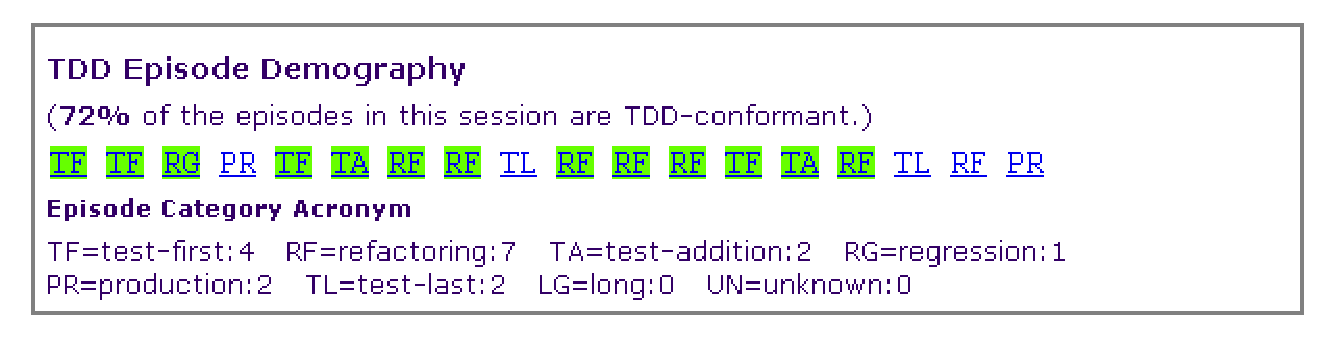
\includegraphics[width=0.80\textwidth]{zorro-episode-demography.eps}
  \caption{Zorro Episode Demography}
  \label{fig:Analysis-Demography}
\end{figure*} 

Zorro provides a number of additional analyses that enable the developer to
understand the impact of TDD practices on their software product and
process.  Figure \ref{fig:Analysis-Ratio} shows how the ratio of test code
to non-test (production) code changes during the course of a development
session.  The horizontal bar at 1.0 represents equal amounts of test and
production code.  This figure illustrates a scenario of initial module
development in which there was significantly more production code than test
code at the beginning of the session, but the proportion of test code rose
until it doubled the amount of production code, before returning to 1.5
times the production code at the end of the session.

\begin{figure*}[th]
  \center
  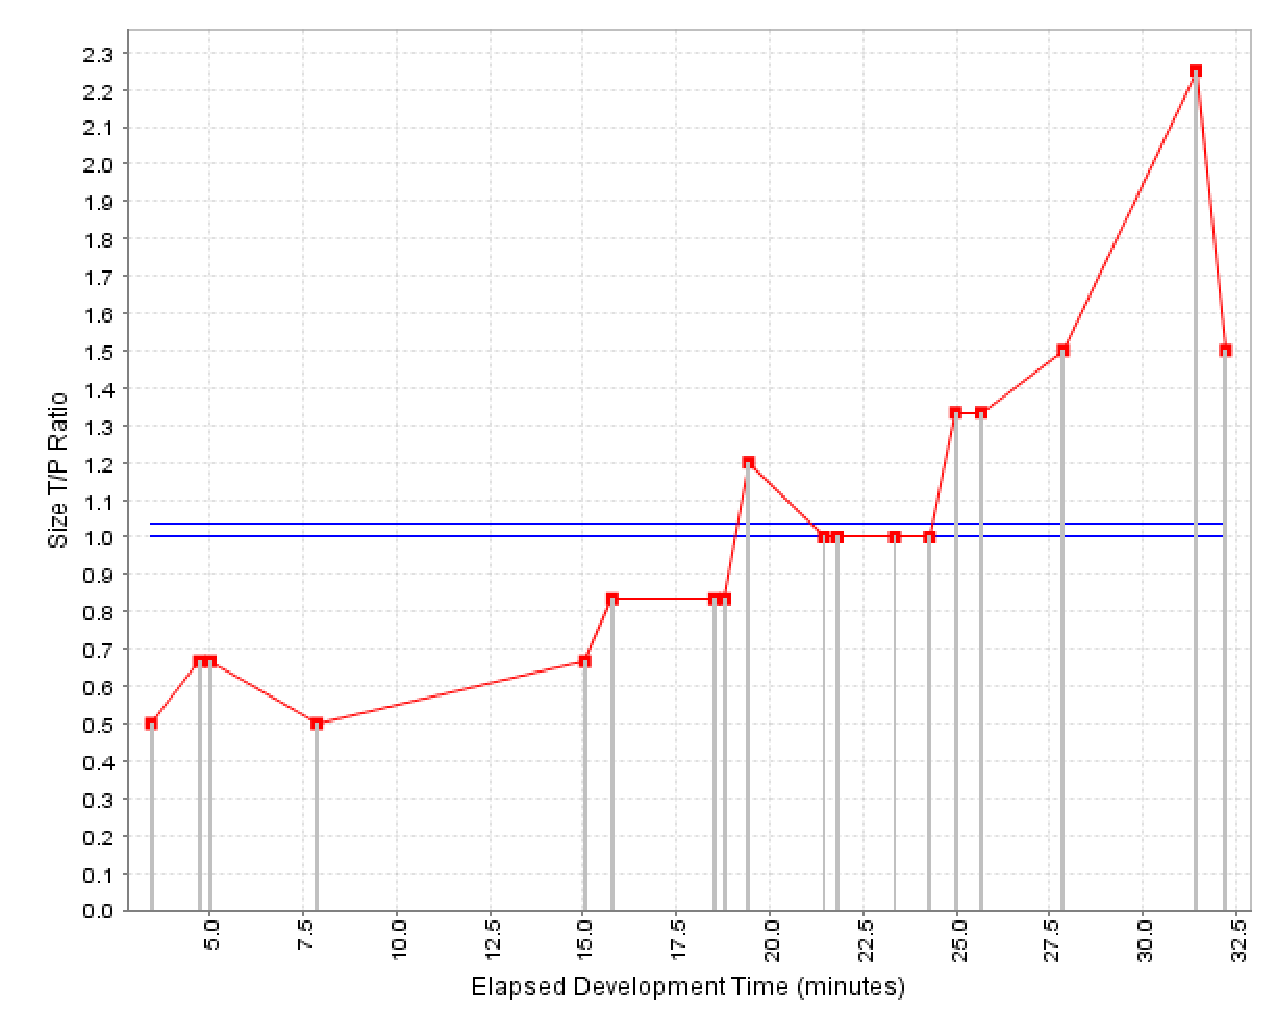
\includegraphics[width=0.80\textwidth]{zorro-test-production-size-ratio.eps}
  \caption{Zorro Test/Production Size Ratio}
  \label{fig:Analysis-Ratio}
\end{figure*} 

The final example analysis illustrated in Figure
\ref{fig:Analysis-Telemetry} pops up to yet another level of abstraction by
using Software Project Telemetry, a capability of Hackystat that enables
the visualization of trends in process and product data over days, weeks,
or months.  In this real world data, two trends are displayed over the
course of eight weeks: the percentage of TDD conforming episodes, and the
test case coverage of the system under development.  Interestingly, the
level of test case coverage co-varies with the ``level'' of TDD practiced
by the developer.

\begin{figure*}[th]
  \center
  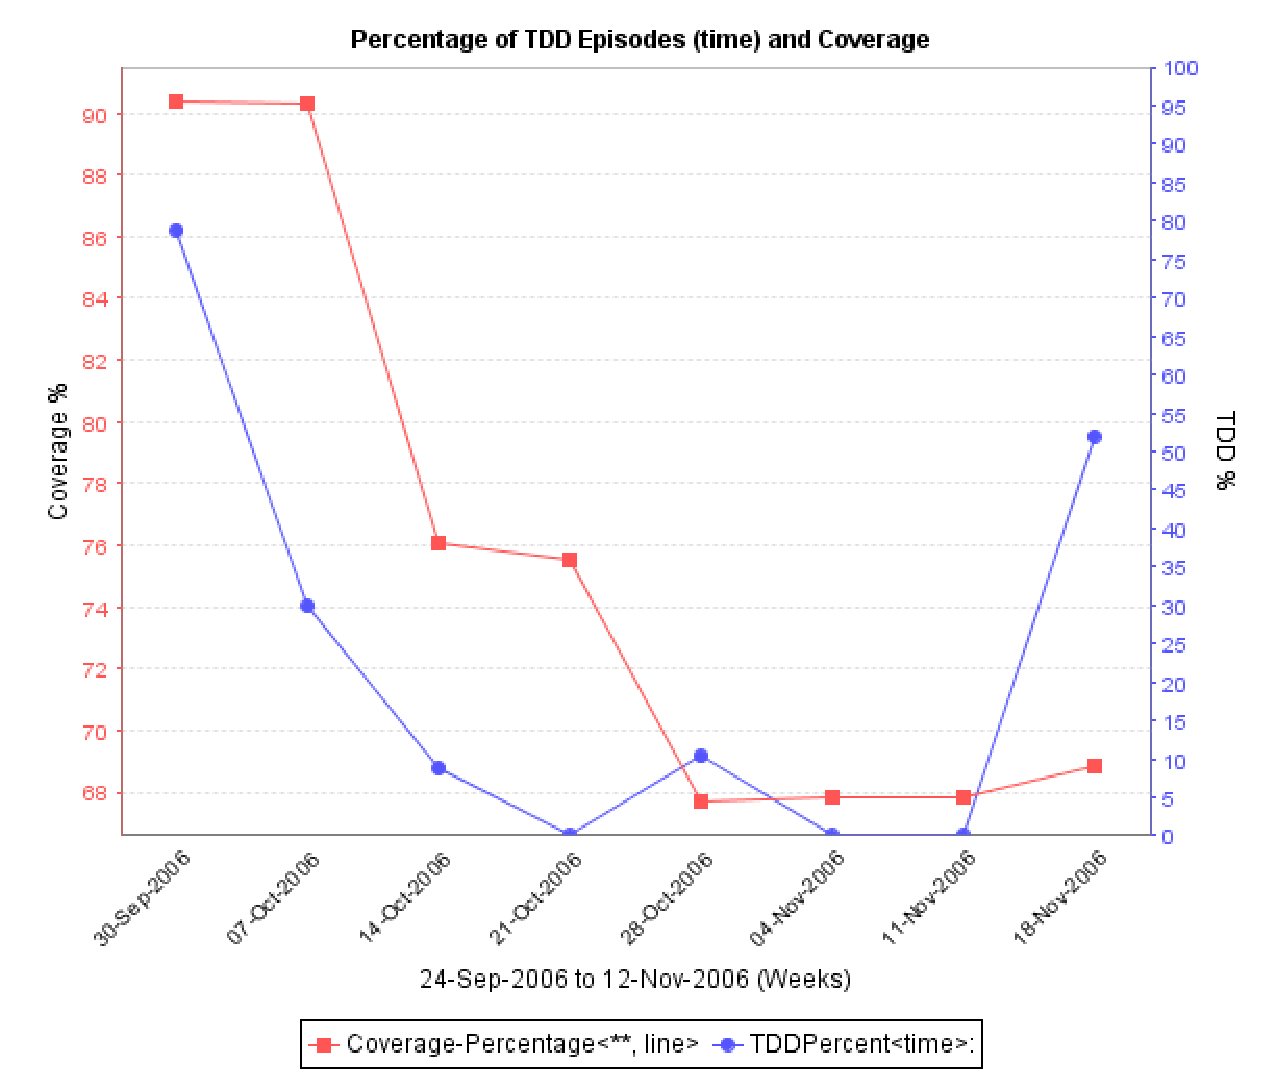
\includegraphics[width=0.80\textwidth]{zorro-tdd-coverage-2.eps}
  \caption{Zorro TDD Episode Telemetry}
  \label{fig:Analysis-Telemetry}
\end{figure*} 


\section{Validation}
\label{sec:validation}

In order to feel confident in Zorro as an appropriate tool to investigate
TDD, we must address two basic validation questions: (1) Does Zorro collect
the behaviors necessary to determine when TDD is occurring, and (2) Does
Zorro correctly recognize test-driven development when it is occurring?

The first validation issue addresses the use of automated, unobtrusive,
sensor-based data collection, and whether this approach can actually
acquire the data necessary to determine when TDD is taking place.

The second validation issue addresses our operational definition of TDD
based upon episode-based classification, and whether it provides a robust,
useful, and acceptable definition of TDD.

We began Zorro validation in the Spring of 2006 with a pilot study, and 
are building on that initial work in 2007.

\subsection{The pilot validation study}

To obtain some initial validation data on Zorro, we conducted a pilot study
in Spring of 2006 in which we instrumented the development environment with
Zorro sensors, asked a small set of students to do some simple TDD
development, then compared the resulting Zorro TDD classifications to an
independently collected source of data regarding their development
behaviors.

One approach to independent data collection would be to have an observer
watching the developers as they programmed, taking notes as to whether they
are performing TDD or not.  We considered this but discarded it as
unworkable: given the rapidity with which TDD cycles can occur, it would be
quite hard for an observer to notate all of the TDD-related events that can
occur literally within seconds of each other. We would end up having to
validate our validation technique!

Instead, we developed a plugin to Eclipse called the ``Eclipse
Screen Recorder'' (ESR).  This system generates a Quicktime movie
containing time-stamped screen shots of the Eclipse window at regular
intervals. One frame/second was found to be sufficient for validation,
generating file sizes of approximately 7-8 MB per hour of video.  The
Quicktime movie created by ESR provides a visual record of developer
behavior that can be manually compared to the Zorro analysis using the
timestamps and used to answer the two validation questions.

Our pilot validation study involved the following procedure. First, we
obtained agreement from seven volunteer student subjects to participate in
the pilot study. These subjects were experienced with both Java development
and the Eclipse IDE, but not necessarily with test-driven development.
Second, we provided them with a short description of test-driven design,
and a sample problem to implement in a test-driven design style.  The
problem was to develop a Stack abstract data type using test-driven design,
and we supplied them with an ordered list of tests to write and some sample
test methods to get them started.  Finally, they carried out the task using
Eclipse with both ESR and Zorro data collection enabled.

To analyze the data, we created a spreadsheet in which we recorded the
results of watching the Quicktime movie and manually encoding the developer
activities that occurred.  Then, we ran the Zorro analyses, added their
results to the spreadsheet, and validated the Zorro classifications against
our analysis of the video record.

The participants spent between 28 and 66 minutes to complete the task.
Zorro partitioned the overall development effort into 92 distinct episodes,
out of which 86 were classified as either Test-Driven, Refactoring, or
Test-Last; the remainder were ``unclassified'', which normally corresponded
to startup or shutdown activities.  Note that the version of Zorro used in
Spring 2006 used a somewhat less sophisticated classification ruleset than
the current version.

Out of the 92 episodes under study, 82 were validated as correctly
classified, for an accuracy rate of 89\%.

\subsection{Ongoing validation}

The pilot study provided us with valuable feedback about the potential
utility of Zorro, as well as deeper insight into the process of validation
itself.  Our current research is focused on enhancing our understanding of
the strengths and weaknesses of Zorro with several additional validation
studies.

Our next validation study will also involve students, and will expand on
the pilot study by cross-validating the Zorro operational definition of TDD
against two independent data sources: the ESR video stream and the feedback
of the participants themselves following the TDD development session.  We
will ask them to review the TDD episodes generated by Zorro and provide
their personal feedback on the classifications.

Following this second student-based validation study, we plan to gain
insight into the strengths and weaknesses of Zorro in professional
settings.  For this case study, we will invite developers who
practice TDD and who use Eclipse, Java, and JUnit to help us validate
Zorro.  The process involves installing the Hackystat Eclipse sensor for
Zorro into their development environment, performing development for a few
days with the sensors installed, then reviewing the classifications made by
Zorro and providing us with feedback regarding its accuracy.

We also plan to obtain feedback from the TDD research community.  We believe
that Zorro can provide useful infrastructure for research on test driven
development.  For this case study, we will invite researchers to 
evaluate Zorro against their experimental requirements and provide us with 
feedback as to the suitability of Zorro for their own work. 

\section{Conclusions}
\label{sec:conclusions}

TDD has great potential as a software development technique, but to fully
realize this potential, the software development community must gain deeper
insight into its strengths and weaknesses.  The Zorro system shows how it
is possible to define an operational definition of Test Driven Development
that can be used to address the process conformance problem and other
methodological issues confronting researchers in TDD.  Zorro also enables
TDD to be analyzed and understood with more precision and nuance than ever
before: instead of red-green-refactor, one can now talk about the
percentage of TDD episodes and which of 22 episode types have been used.
When combined with other Hackystat analysis techniques such as Software
Project Telemetry, Zorro enables developers to gain deeper empirical
insight into how TDD practice impacts on other process and product metrics,
such as test case size and coverage.

In our experience, however, Zorro is more than simply an experimental
infrastructure or a TDD learning device.  Zorro demonstrates that it is now
possible to observe and analyze interesting ``micro-processes'' in software
development.  By building Zorro on top of the more generic SDSA and
Hackystat frameworks, its architecture makes it more easily possible to
study not only TDD, but other interesting developer ``best practices'' on
this fine-grained level.  For example, there are many best practices
surrounding the appropriate time to commit file changes to a configuration
management repository, and at least some of these best practices could be
operationalized in a set of Hackystat sensors and SDSA rules. 

Finally, we want to emphasize the open source nature of the Zorro system and 
the research process.   We encourage you to download the system and try it out,
or contact us if you wish to participate in the research process. 

\bibliographystyle{latex8}
\bibliography{tdd,zorro,csdl-trs,hackystat,psp}
\end{document}











